% Requires:
% \usepackage{pgfplots}
% \pgfplotsset{compat=1.18}

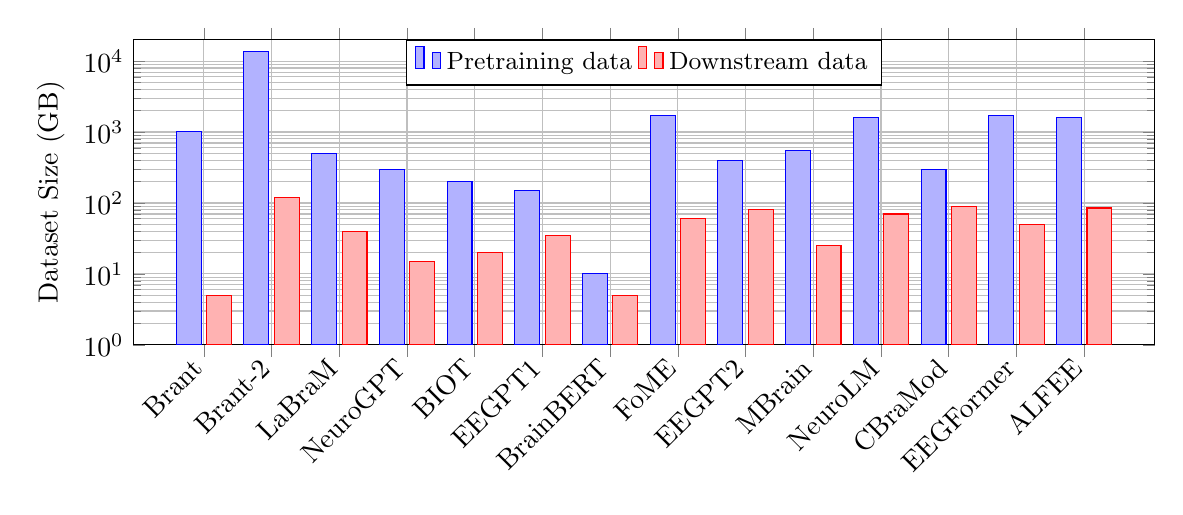
\begin{tikzpicture}
    \begin{axis}[
            ybar,
            width=\linewidth,
            height=0.45\linewidth,
            ylabel={Dataset Size (GB)},
            ymode=log,
            ymin=1,
            x=0.86cm,
            ymax=20000,
            log basis y={10},
            symbolic x coords={
                    Brant,
                    Brant-2,
                    LaBraM,
                    NeuroGPT,
                    BIOT,
                    EEGPT1,
                    BrainBERT,
                    FoME,
                    EEGPT2,
                    MBrain,
                    NeuroLM,
                    CBraMod,
                    EEGFormer,
                    ALFEE
                },
            xtick=data,
            x tick label style={rotate=45, anchor=east},
            bar width=9pt,
            enlarge x limits=0.08,
            grid=both,
            legend style={
                    at={(0.5,0.85)},
                    anchor=south,
                    legend columns=2,
                    font=\small
                }
        ]

        % Pretraining dataset size (GB, approximate from Table I / text)
        \addplot coordinates {
                (Brant,1010)
                (Brant-2,13790)
                (LaBraM,500)
                (NeuroGPT,300)
                (BIOT,200)
                (EEGPT1,150)
                (BrainBERT,10)
                (FoME,1700)
                (EEGPT2,400)
                (MBrain,550)
                (NeuroLM,1600)
                (CBraMod,300)
                (EEGFormer,1700)
                (ALFEE,1600)
            };
        \addlegendentry{Pretraining data}

        % Downstream dataset size (GB-equivalent, indicative)
        \addplot coordinates {
                (Brant,5)
                (Brant-2,120)
                (LaBraM,40)
                (NeuroGPT,15)
                (BIOT,20)
                (EEGPT1,35)
                (BrainBERT,5)
                (FoME,60)
                (EEGPT2,80)
                (MBrain,25)
                (NeuroLM,70)
                (CBraMod,90)
                (EEGFormer,50)
                (ALFEE,85)
            };
        \addlegendentry{Downstream data}

    \end{axis}
\end{tikzpicture}
